\documentclass[12pt]{report}
\usepackage[utf8x]{inputenc}
\usepackage{graphicx}
\usepackage{textcomp, gensymb}
\usepackage{gensymb}
\usepackage{amssymb}
\usepackage{algorithm}
\usepackage[noend]{algpseudocode}
\usepackage{algpseudocode}
\graphicspath{{./images}}
\usepackage{fancyhdr}
\usepackage{blindtext}
\usepackage[colorlinks=true, urlcolor=black, linkcolor=black]{hyperref}
\hypersetup{
colorlinks=true,
linkcolor=black,
urlcolor=black
}
\usepackage{url}


\title{ETERNITY:FUNCTION F4}
\author{Tavtej Singh Lehri}
\date{}
\newcommand*{\Gtr}{\smallrel\gtr}

\makeatletter
\let\thetitle\@title
\let\theauthor\@author
\let\thedate\@date
\makeatother

\fancypagestyle{}{}
\fancyhf{}
\rhead{\thetitle}
\cfoot{\thepage}

\begin{document}

\begin{titlepage}
\centering
\vspace*{0.5 cm}

\begin{center}
\textsc{\Large CONCORDIA UNIVERSITY}\\ [2.0 cm]    
\end{center}

\textsc{\large SOEN 6011: Software Engineering Processes}\\[0.5 cm]
\rule{\linewidth}{0.2 mm}\\[0.4 cm]
{\LARGE \textbf \thetitle}\\[0.2 cm]
{\LARGE \textbf{$\Gamma$(x)}}
\rule{\linewidth}{0.2 mm}\\[1.5 cm]

\begin{center}
    {\Large \textbf{\theauthor}}\\[0.2 cm]
    {\large Student ID: 40121745}\\[2.0 cm]
    
    \begin{figure}[h!]
    \begin{center}
    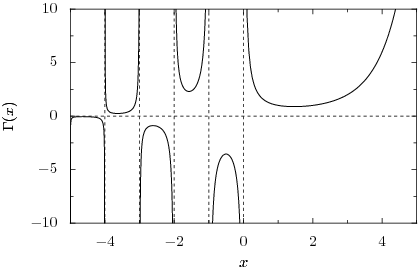
\includegraphics[width=0.5\linewidth]{Gamma_function.png}
    \end{center}
    \caption{Graph of Gamma Function.\cite{gamma}}
    \end{figure}
    
    {\large \url{https://github.com/tavtejS07/SOEN-6011}}
\end{center}

\end{titlepage}

\tableofcontents
\pagebreak

\renewcommand{\thesection}{\arabic{section}}
\section{Problem 1}
\subsection{Description}
Gamma function is said to be an extension of the factorial function used for complex numbers. For any positive integer Gamma function is defined as below.

\begin{equation}
\Gamma(x) = (x-1)\Gamma(x-1)\\
   \Rightarrow \Gamma(x) = (x-1)!
\end{equation}
\newline
\textbf{Definition: }The function which is improper integral of another function is defined as Gamma function.\cite{libretexts} Using the integral formula below we can define Gamma function. \textbf{Note: }For all positive real number x{(i.e $Re(x)>0$)}, the integral follows absolute convergence.\cite{libretexts} This was derived by \textbf{Daniel Bernoulli}.
\begin{equation}
    \Gamma(x) = \int\limits_0^\infty t^{x-1} e^{-t} dt\
\end{equation}

\subsection{Characteristics}
\begin{enumerate}
    \item $\Gamma(x)$ is defined and analytic for it's domain.\cite{libretexts}
    \item $\Gamma(x)$ displays the recursive property for $x>0$. This is displayed in equation 1 above.
    \item $\Gamma(x)$ is a meromorphic function, with $\mathbb{Z}\leq0$ as poles.\cite{gamma}
\end{enumerate}


\subsection{Domain}
Set of positive real numbers.
$x\in\mathbb{R}$ and  $x>0$
\subsection{Co-Domain}
For a specific domain, co-domain for Gamma function is
\begin{displaymath}
    \mathbb{R}>0 = \{x\in\mathbb{R}|x>0\}
\end{displaymath}

\section{Problem 2}
\subsection{Assumptions}

\subsubsection{Assumption 1}
\begin{itemize}
    \item \textbf{ID = }Gamma\_Asump\_01
    \begin{itemize}
        \item Input for the function $\Gamma(x)$ is a real number, where $\mathbb{R}>0.$
    \end{itemize}
\end{itemize}

\subsubsection{Assumption 2}
\begin{itemize}
    \item \textbf{ID = }Gamma\_Asump\_02
    \begin{itemize}
        \item At no point is the value of $\Gamma(x) = 0$
    \end{itemize}
\end{itemize}

\subsubsection{Assumption 3}
\begin{itemize}
    \item \textbf{ID = }Gamma\_Asump\_03
    \begin{itemize}
        \item For the input values which are not within the domain, system throws an error and we get an undefined result.
    \end{itemize}
\end{itemize}


\subsection{Functional Requirements}
\subsubsection{Requirement 1}
\begin{itemize}
    \item \textbf{ID = }Gamma\_FR\_001
    \item \textbf{Type = }Functional Requirement
    \item \textbf{Version = } 1.0
    \item \textbf{Difficulty = }High
    \item \textbf{Description = } All the inputs should be within the domain. If the value lies outside the domain, error should be thrown by the system.
\end{itemize}

\subsubsection{Requirement 2}
\begin{itemize}
    \item \textbf{ID = }Gamma\_FR\_002
    \item \textbf{Type = }Functional Requirement
    \item \textbf{Version = } 1.0
    \item \textbf{Difficulty = }High
    \item \textbf{Description = } All the inputs which are positive integers should calculate the factorial of that integer. This will be the output of gamma function.
    \item \textbf{Rationale = }As gamma function follows recursive property for $\mathbb{Z}>0.$ $\Gamma(x)=(x-1)\Gamma(x-1)$
\end{itemize}

\subsubsection{Requirement 3}
\begin{itemize}
    \item \textbf{ID = }Gamma\_FR\_003
    \item \textbf{Type = }Functional Requirement
    \item \textbf{Version = } 1.0
    \item \textbf{Difficulty = }Medium
    \item \textbf{Description = } User should provide a single input only.
    \item \textbf{Rationale = }input is either a non-negative integer or a real number greater than 0.
\end{itemize}

\newpage
\section{Problem 3}
\subsection{Algorithms}
\begin{algorithm}
\caption{Lanczos Approximation for StrictMath}
\begin{algorithmic}[1]
\If{$x$ is negative or is $NaN$}
\State $NaN$
\EndIf
\If{$x$ is equal to 0}
\State \textbf{return} $1$
\EndIf
\If{$x$ is greater than 0}
\State $double$ $d = (x-0.5) * log(x+4.5) - (x+4.5)$
\State $double$ $e = 1.0 + X1/(x+0) - X2/(x+1) + X3/(x+2) - $
\State $X4/(x+3) + X5/(X+4) - X6/(x+5)$
\State \textbf{return} $d + log(d1 * sqrt(2*\pi)) --> logGamma$
\EndIf
\State \textbf{Using the value returned in Line 9 calculate $\Gamma(x)$}
\State \textbf{return} $exp(logGamma(x))$

\end{algorithmic}
\end{algorithm}

\begin{algorithm}
\caption{Stirling's Approximation for StrictMath}
\begin{algorithmic}[1]
\If{$x$ is negative or is $NaN$}
\State $NaN$
\EndIf
\If{$x$ is equal to 0}
\State \textbf{return} $1$
\EndIf
\If{$x$ is greater than 0}
\State \textbf{return}
sqrt(2*$\frac{\pi}{x}$)*($\frac{x}{e}$)$^x$
\EndIf
\end{algorithmic}
\end{algorithm}

\subsection{Technical Aspects}
Algorithm 1 is Lanczos approximation of the function $\Gamma(x).$ This is an alternative to the Stirling's approximation. The advantage of this is the less number of single or double floating point precision required. If a real constant is known then we can easily calculate the coefficients in advance and use a single formula.\\
\newline
Algorithm 2 is the approximation of factorials. It has Big Oh! of O(nlogn). Calculation factorial for larger numbers take time if we implement n!. Using the Stirling's approximation it reduces the time of calculation.

\section{Problem 4}
\subsection{Debugger}
 \begin{figure}[h!]
    \begin{center}
    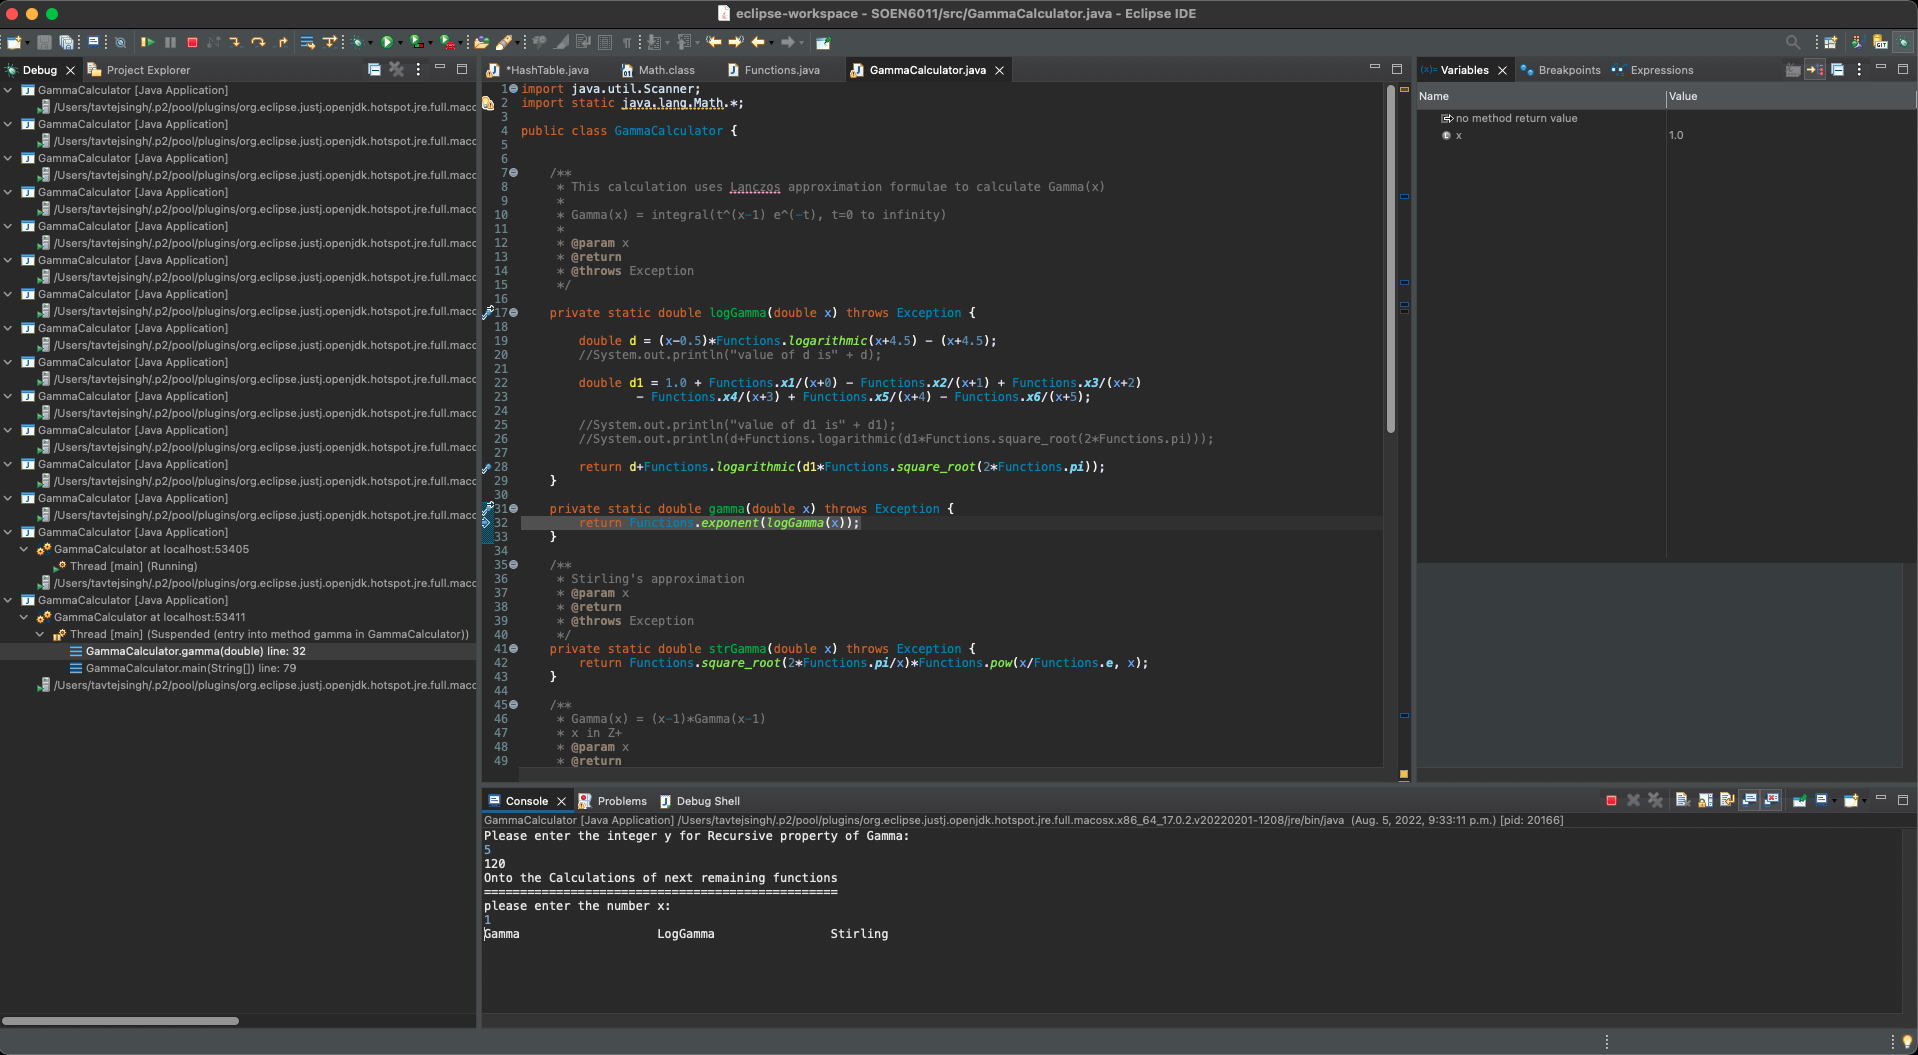
\includegraphics[width=1.0\linewidth]{Debugger.png}
    \end{center}
    \caption{Debugger Eclipse.}
 \end{figure}

The purpose of debugger is to run the program interactively. One can view the variable by variable execution in the debugging perspective. For the program ANT debugger was used which has features such as Breakpoints, Variable tracking, parameter specification and so on.

\newpage
\subsection{Checkstyle}

\begin{figure}[h!]
    \begin{center}
    \includegraphics[width=0.7\linewidth]{Checkstyle1.png}
    \end{center}
    \caption{Checkstyle Eclipse.}
 \end{figure}
 
 \begin{figure}[h!]
    \begin{center}
    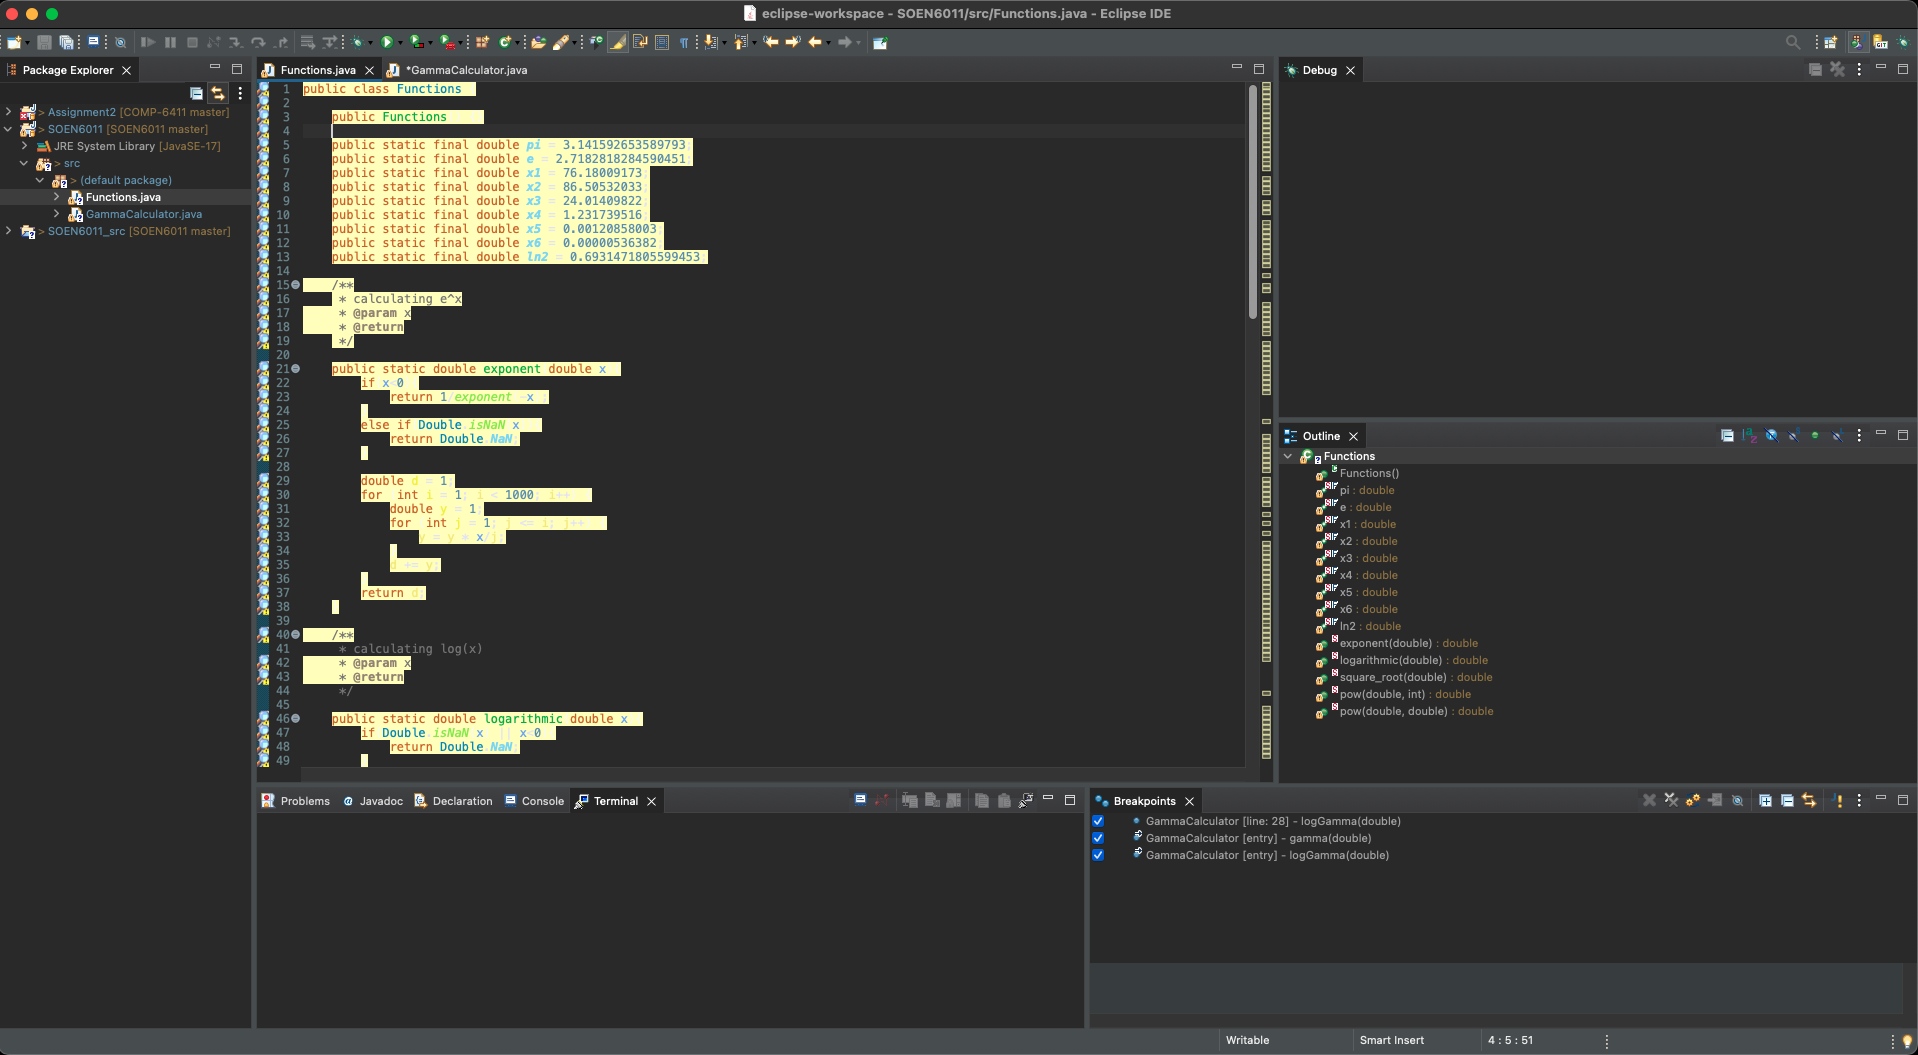
\includegraphics[width=0.7\linewidth]{Checkstyle2.png}
    \end{center}
    \caption{Checkstyle Eclipse.}
 \end{figure}


\begin{thebibliography}{9}
\addcontentsline{toc}{chapter}{Bibliography}
\bibitem{libretexts}
Libretexts. (2022, February 27). \textit{E14.2: Definition and properties of the gamma function.}Mathematics LibreTexts. Retrieved July 25, 2022, from \texttt{https://math.libretexts.org/Bookshelves/Analysis/\\Complex\_Variables\_with\_Applications\_(Orloff)/14\%3A\_Analytic\_Continuation\_\\and\_the\_Gamma\_Function/14.02\%3A\_Definition\_and\_properties\_of\_the\_Gamma\_function}

\bibitem{gamma}
Gamma function. (2011, July 25). \textit{Gamma function}- Knowino. (n.d.). Retrieved July 27, 2022, from\\ \texttt{https://www.tau.ac.il/~tsirel/dump/Static/knowino.org/wiki/Gamma\_function.html}

\bibitem{code}
The Trustees of Princeton University. (n.d.). \textit{Gamma.java.} Princeton University. Retrieved August 5, 2022, from \texttt{https://introcs.cs.princeton.edu/java/91float/Gamma.java.html }

\end{thebibliography}

\end{document}